\problemname{Mancala}

\begin{figure}[p]
    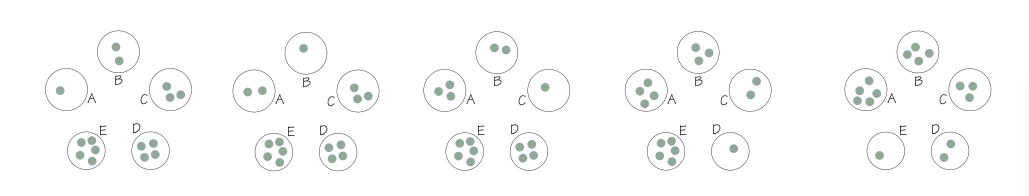
\includegraphics{figur.png}
	\caption{Sample 1}
\end{figure}

\emph{Mancala} is an ancient game from Africa, from which we borrow the principles in this problem. The figure above shows 5 positions. In each position, we see 5 \emph{bowls} containing a varied number of \emph{seeds}. On the far left, we see an example of a \emph{starting position} and on the far right, an example of a desired \emph{ending position}. To reach the ending position, 4 moves are needed.

A move consists of the following parts:
\begin{enumerate}
	\item Choose a bowl and pick up all seeds in it.
	\item Choose a direction, \emph{clockwise} or \emph{counterclockwise}.
	\item \emph{Sow} first one seed in the bowl you just emptied. Then sow one seed in each bowl, in the chosen direction, as far as they last.
\end{enumerate}

Then repeat steps 1--3 until the desired ending position is reached.

In the example in the figure, the following moves are made: First we choose bowl B and sow counterclockwise. In the next move, we choose bowl C and again sow counterclockwise. In the third move, we choose bowl D and direction counterclockwise. In the fourth and final move, we pick up the seeds from bowl E. Now we can choose any direction; the result is the same either way. Thus, from the starting position 1, 2, 3, 4, 5 we have reached the ending position 5, 4, 3, 2, 1 in four moves (the bowls' contents are presented in the order A, B, C, D, E).

Write a program that receives a starting position and an ending position and determines the minimum number of moves required to reach the goal. In our tests, no more than 6 moves will ever be needed.

The maximum number of seeds in a bowl in the starting position is 10.

\section*{Input}
The input consists of two lines. The first line contains the starting position as 5 space-separated integers with the number of seeds in the bowls (in the order A, B, C, D, E). The second line contains the ending position, presented in the same way. No bowl contains more than 10 seeds.

\section*{Output}
Output a single integer: the minimum number of moves needed to reach the ending position.
